% TODO ??

During the development process of \myTitle the first issue that need to be
resolved was the description of a suitable model for supporting such framework.
The design of a model involves the definition of the data structures that will
be used by the workflow, and of course the definition of the workflow itself.

\subsection{Data Design}
% durante il design abbiamo dovuto tener conto del problema che dovevamo risolvere
% data la flessibilità e generalità di questo 
% abbiamo desciso di usare un metamodello
% il metamodello voveva essree in grasdo di supportare i processi descritti più avanti
%  pluggabilità
In the design process for the data model we faced the problem of creating a
suitable underlying model for all the application need that we have to cover,
spacing from pure \acl{HC} task to \emph{parasitic computing}. This wide range
of possible application and the need of great flexibility demanded to the system,
led us to the creation of a meta model for almost all the data structures used in
the framework. The metamodel was subdivided in four: the \emph{Workflow}, the
\emph{Task Data Model}, the \emph{Task Model} and the \emph{Task Execution Model}.

\paragraph{The Workflow Model} describes the flow of the execution of the Task
within the framework, the relationships that needs to be taken into account to
correctly execute a sequence of task (called \emph{Work}).

\paragraph{The Task Data Model} describes the data model for each Task, including,
if present, the field dependencies and if a field belongs to the input or the
output set.

\paragraph{The Task Model} describes the actual data of the Task, called
\emph{Objects}, for the Task.

\paragraph{The Task Execution Model} describes the actual execution step for
each Task, providing information on which user is performing which task, as long
as data associated to the execution itself.


\subsection{Workflow Design}\label{design:work}
\begin{figure}[htb]
    \centering
    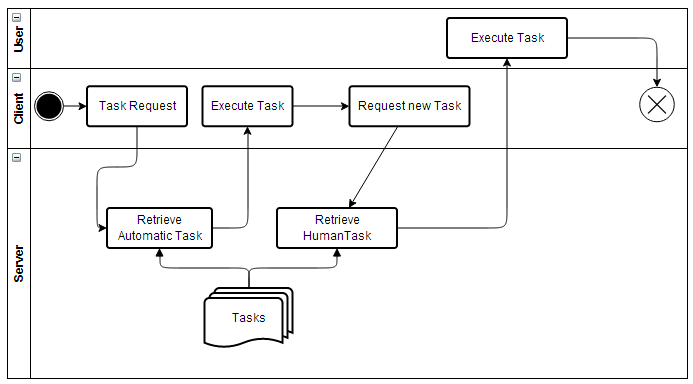
\includegraphics[width=\columnwidth]{Workflow}
    \caption{The conceptual Workflow handled by the framework.}
    \label{fig:workflow}
\end{figure}
% TODO flow of execution with both human and machine computation
In the \emph{Workflow Design} we must describe, at conceptual level, how our
framework deal with the client and how the task are executed. During the
\emph{Data Design} we stated that the tasks can have relationships and thus our
framework must be able to handle different Task types seamlessly. In
\autoref{fig:workflow} is depicted a typical flow of execution of a Work (a
composition of Tasks) with multiple task types.\\

Our Workflow model must be able to handle the interleaving of human and automatic
task without any human intervention. The Workflow must take into account also the
constraints defined during the creation step and manage the execution of the
tasks accordingly.

A feature that the framework is required to handle is also the case where
the application type is not strictly human or strictly automatic. We can have
scenarios where the task is a blend of both human and automatic interactions.
\ac{GWAP} are a case where the automatic computation and the human interaction
are blended together. Other scenarios can be the validation of the automatically
computed results as we presented in our use case (see \ref{sec:cases:hybrid}).

To guarantee the needed flexibility the framework must be able to include third-part
logic in charge of managing certain steps of the execution (like Task planning).




\subsection{Framework Design}
% come sono arrivato all'architettura del framework
In the design of the framework all the conceptual designed data and workflows as
long as the requirements are merged and adapted to create the whole structure for
supporting the framework.\\

During the \textbf{Data Design} we pointed out the data structures that
need to be managed. The \emph{Workflow Model} need to specify the relationship
between the modules an the "connection points" where the third part softwares
are plugged. On top of that every Task must have defined its set of input and
output data.
The \emph{Task Data Model} specifies all the data structure of the task, building
the metamodel for each Task. The metamodel contain all the information on the 
structure of the data model for a Task.
In the \emph{Task Model} are contained all the actual data for each Task, called
Objects, each object represents a "row" of the data. Each object is, in turn,
associated to a Task.
The \emph{Task Execution Model} contains all the information on the actual
execution of a Task, keeping information on the user that performer the task and
the used device, if any.\\

The \textbf{Workflow Design} allow us to create the software able to handle all
the different types of archetype application (e.g. Human computation, Automatic
computation) giving also the guidelines on how to manage the interaction between
subsequent Task execution.